\interlude[0]{The design of Rosenpass \\ \vspace{0.8em} \small and how to build post-quantum protocols}
\section{The design of Rosenpass}

\begin{frame}[light]{In the following slides, you will learn…}
  \begin{columns}[c]
    \begin{column}{.40\linewidth}
      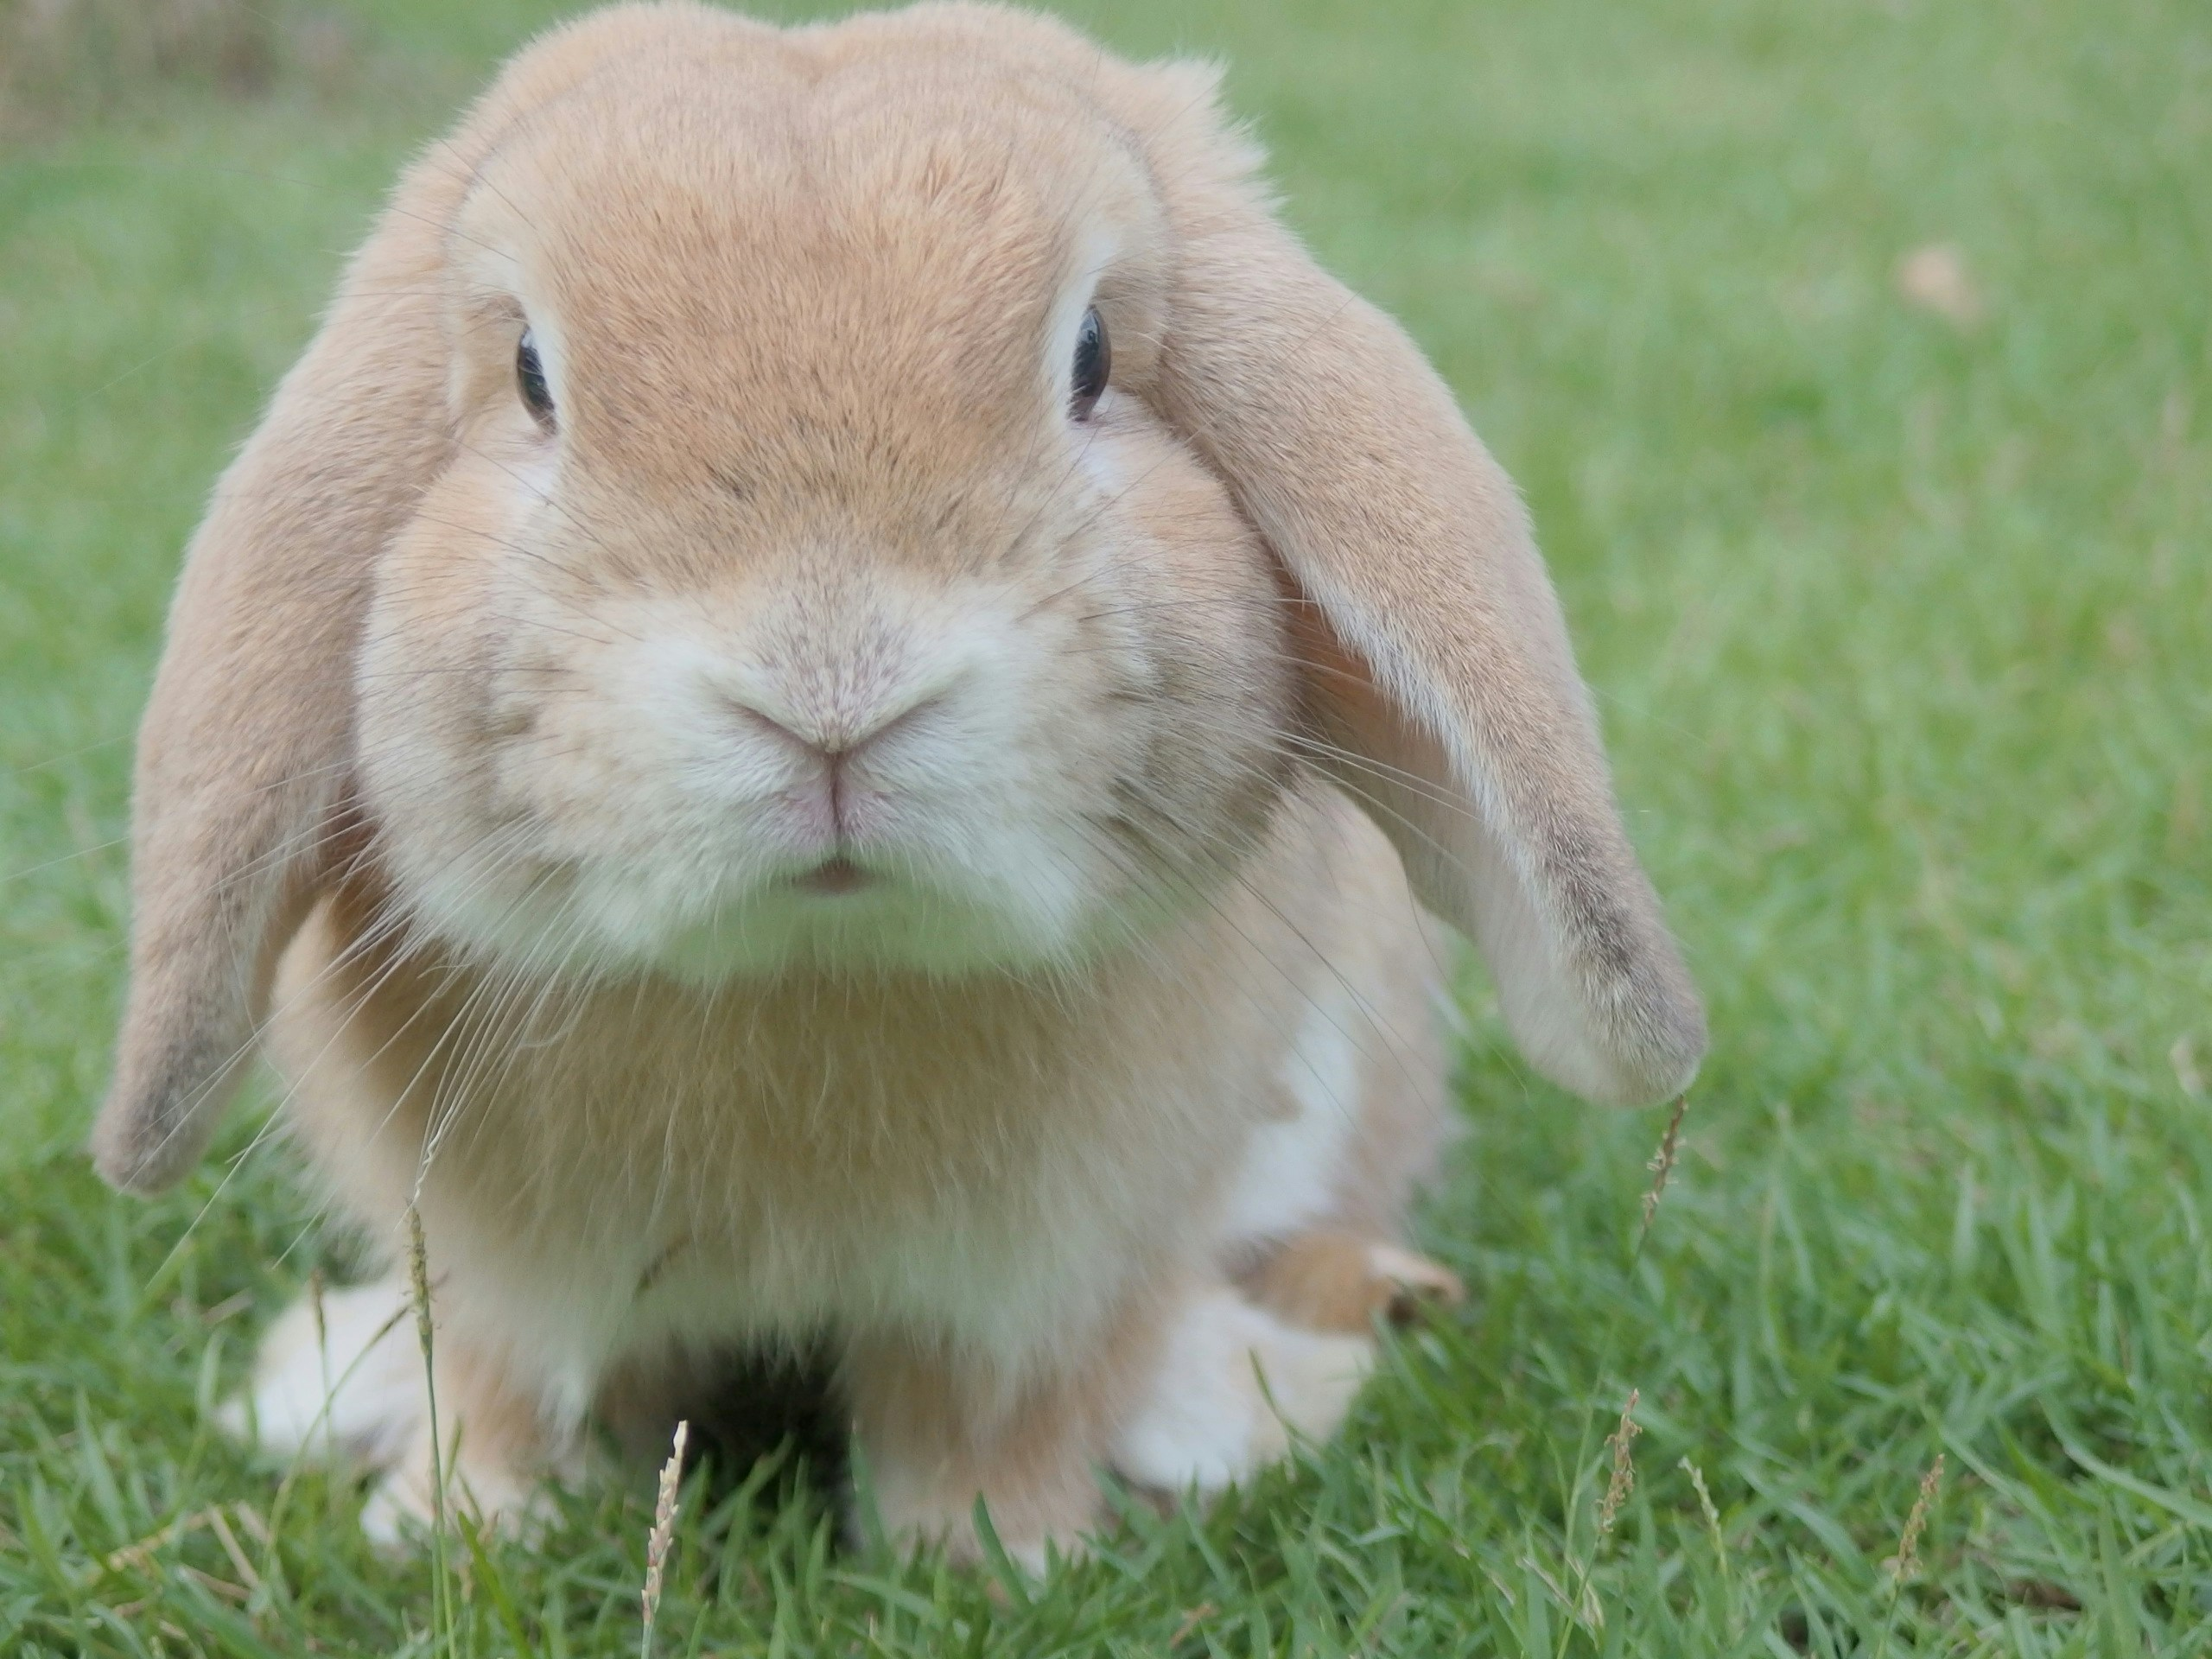
\includegraphics[width=.6\linewidth,right,padding=-.2cm .2cm 0cm .2cm]{graphics/bunny-looking-at-camera.jpg}
      \par
      \includegraphics[width=1.1\linewidth,right]{graphics/coffe-barista-next-to-roaster.jpg}
    \end{column}

    \begin{column}{.60\linewidth}
      …that most cryprographic applications today are susceptible against attacks from quantum computers.

      \vspace{2em}
      …that this is not fundamental to cryptography, but that pre-quantum protocols are simply a more efficient.

      \vspace{2em}
      …that – cryptographically speaking – the difference between pre-quantum and post-quantum crypto is about a subtle
      difference in function interface.
    \end{column}
  \end{columns}
\end{frame}




\begin{frame}{Glossary: Post-quantum security}
\vspace{-\ht\strutbox}
  \begin{columns}[t]
    \begin{column}{.30\linewidth}
      \begin{block}{Pre-quantum Cryptography is… \strut}

      …susceptible to attacks from quantum computers.

      \vspace{0.5em}
      \begin{itemize}
        \item Specifically, to \emph{Shor's Algorithm} % TODO(karolin): Citation needed
        \item Quite fast
        %\item Widely used
        \item Widely widely trusted
      \end{itemize}
      \end{block}
    \end{column}

    \begin{column}{.33\linewidth}
      \begin{block}{Post-quantum cryptography is…}

        …not susceptible to attacks from quantum computers.

      \vspace{0.5em}
      \begin{itemize}
        \item generally less efficient.
        \item much bigger ciphertexts.
        %\item hard to use on embedded devices.
        %\item adoped in the last decade.
        \item less analyzed.
      \end{itemize}
      \end{block}
    \end{column}

    \begin{column}{.36\linewidth}
      \begin{block}{Hybrid cryptography combines…}
        …the combination of the previous two. It is…


        \vspace{0.3em}
        \begin{itemize}
          \item about as inefficient as post-quantum cryptography.
          \item not widely adopted, which is a major problem.
        \end{itemize}
      \end{block}
    \end{column}
  \end{columns}
\end{frame}





\begin{frame}{What post-quantum got}
  \centering
  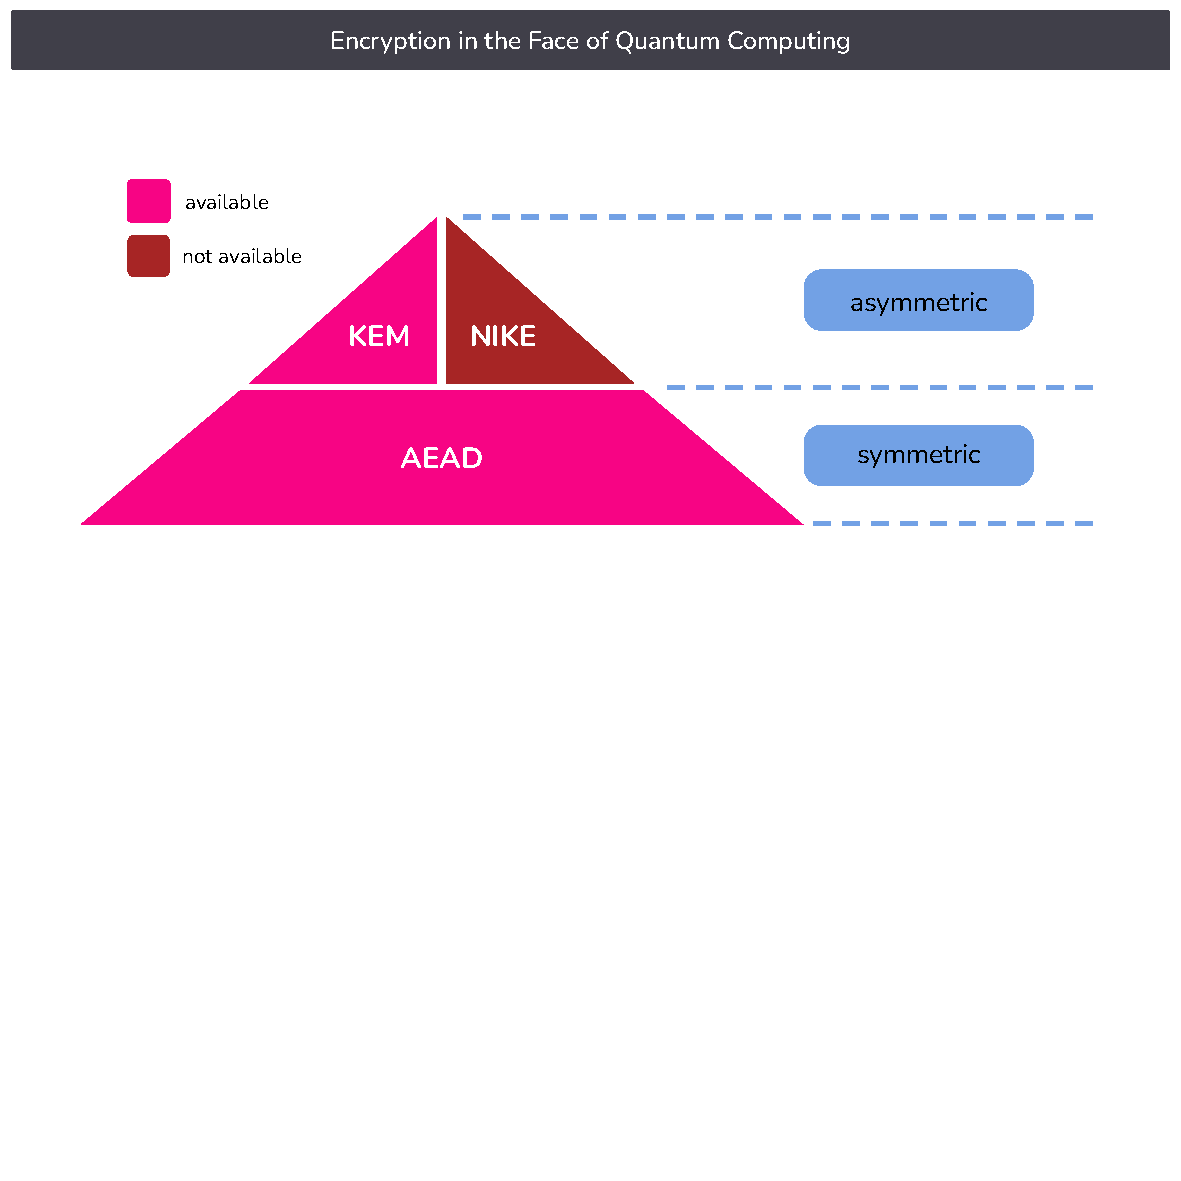
\includegraphics[width=\linewidth,page=1,clip=true,trim=1cm 1cm 0cm 3cm]{graphics/rosenpass-key-exchanges-nike-kem.pdf}
\end{frame}





\begin{frame}[fragile,T]{NIKEs and KEMs}
  \begin{columns}[t,fullwidth]
    \begin{column}{.49\linewidth}
\begin{rustblock}{Key Encapsulation Method}
fn Kem::encaps(Pk) -> (Shk, Ct);
fn Kem::decaps(Pk, Ct) -> Shk;

(shk, ct) = encaps(pk);
assert!(decaps(sk, ct) = shk)
\end{rustblock}
        \vspace{1em}
        Think of it a encrypting a key and sending it
        to the partner.

        \vspace{0.7em}
        \begin{itemize}
          \item Secrecy
          \item Implicit authentication of recipient
            (assuming they have the shared key, they must
            also have their secret key)
        \end{itemize}
    \end{column}\hfill
    \begin{column}{.49\linewidth}
\begin{rustblock}{Non Interactive Key Exchange}
fn nike(sk: Sk, pk: Pk) -> Shk;

assert!(nike(sk1, pk2) = nike(sk2, pk1));
\end{rustblock}

        % TODO(marei): Can you align these using latex instead of empty lines above?
        \vspace{1em}
        Aka. Diffie-Hellman.
        I don't know a good analogy, but ote how the
        keypairs are \emph{crossing over} to each other.

        \vspace{0.7em}
        \begin{itemize}
          \item Secrecy
          \item Mutual authentication
            (for each party: assuming they have the shared key, they must
            also have their secret key)
        \end{itemize}
    \end{column}

  \end{columns}
\end{frame}




\begin{frame}[fragile,T]{NIKEs and KEMs: Key exchange}
  \begin{columns}[t,fullwidth]
    \begin{column}{.49\linewidth}
      \begin{block}{Key Encapsulation Method}
        % TODO(marei): Can you fix this?
        \begin{description}
          \item[\textbf{Responder Authentication}:] Initiator encapsulates key under the responder public key.
          \item[\textbf{Initiator Authentication}:] Responder encapsulates key under the initiator public key.
          \item[\textbf{Forward-secrecy}:] In case the secret keys get stolen, either party generates a temporary
            and has the other party encapsulate a secret under that keypair.

          \vspace{1em}
          \item[How to do this properly?] See Rosenpass. % TODO: Cite
        \end{description}
      \end{block}
    \end{column}
\hfill
    \begin{column}{.49\linewidth}
      \begin{block}{Non Interactive Key Exchange}
        \begin{description}[leftmargin=0cm]
          \item[\textbf{Responder Authentication}:] Static-static NIKE since NIKE gives mutual authentication.
          \item[\textbf{Initiator Authentication}:] Static-static NIKE since NIKE gives mutual authentication.
          \item[\textbf{Forward-secrecy}:] Another nike, involving a temporary keypair.

          \vspace{1em}
          \item[How to do this properly?] See the Noise Protocol Framework. % TODO: Cite
        \end{description}
      \end{block}
    \end{column}

  \end{columns}
\end{frame}




\begin{frame}[fragile,T]{NIKEs and KEMs}
  \begin{columns}[t,fullwidth]
    \begin{column}{.5\linewidth}
\begin{rustblock}{Key Encapsulation Method}
trait Kem {
  // Secret, Public, Symmetric, Ciphertext
  type Sk; type Pk; type Shk; type Ct;
  fn genkey() -> (Sk, Pk);
  fn encaps(pk: Pk) -> (Shk, Ct);
  fn decaps(sk: Pk, ct: Ct) -> Shk;
}
#[test]
fn test<K: Kem>() {
  let (sk, pk) = K::genkey();
  let (shk1, ct) = K::encaps(pk);
  let shk2 = K::decaps(sk, ct);
  assert_eq!(shk1, shk2);
}
\end{rustblock}
    \end{column}%
    \begin{column}{.5\linewidth}
\begin{rustblock}{Non Interactive Key Exchange}
trait Nike {
  // Secret, Public, Symmetric
  type Sk; type Pk; type Shk;
  fn genkey() -> (Sk, Pk);
  fn nike(sk: Sk, pk: Pk) -> Shk;
}
#[test]
fn test<N: Nike>() {
  let (sk1, pk1) = N::genkey();
  let (sk2, pk2) = N::genkey();
  let ct1 = N::nike(sk1, pk2);
  let ct2 = N::nike(sk2, pk1);
  assert_eq!(ct1, ct2);
}
\end{rustblock}
    \end{column}

  \end{columns}
\end{frame}




\begin{frame}{Rosenpass Kex Exchange Parts}
  \centering
  \includegraphics[width=.9\linewidth,page=6,clip=true,trim=1cm 4cm 0cm 2cm]{graphics/rosenpass-key-exchanges-nike-kem.pdf}
\end{frame}




% \begin{frame}{Rosenpass Unified Key Exchange}
%   \centering
%   \begin{columns}[fullwidth,c]
%     \begin{column}{.6\linewidth}
%       \includegraphics[width=1.3\linewidth,page=7,clip=true,trim=1cm 4cm 0cm 2cm]{graphics/rosenpass-key-exchanges-nike-kem.pdf}
%     \end{column}%

%     \begin{column}{.4\linewidth}
%       \includegraphics[width=\linewidth,page=5,clip=true,trim=3cm 7cm 0cm 3.5cm]{graphics/rosenpass-key-exchanges-nike-kem.pdf}
%     \end{column}
%   \end{columns}
% \end{frame}





\begin{frame}{Rosenpass Protocol Features}
  \begin{columns}[fullwidth,c]
    \begin{column}{.6\linewidth}
      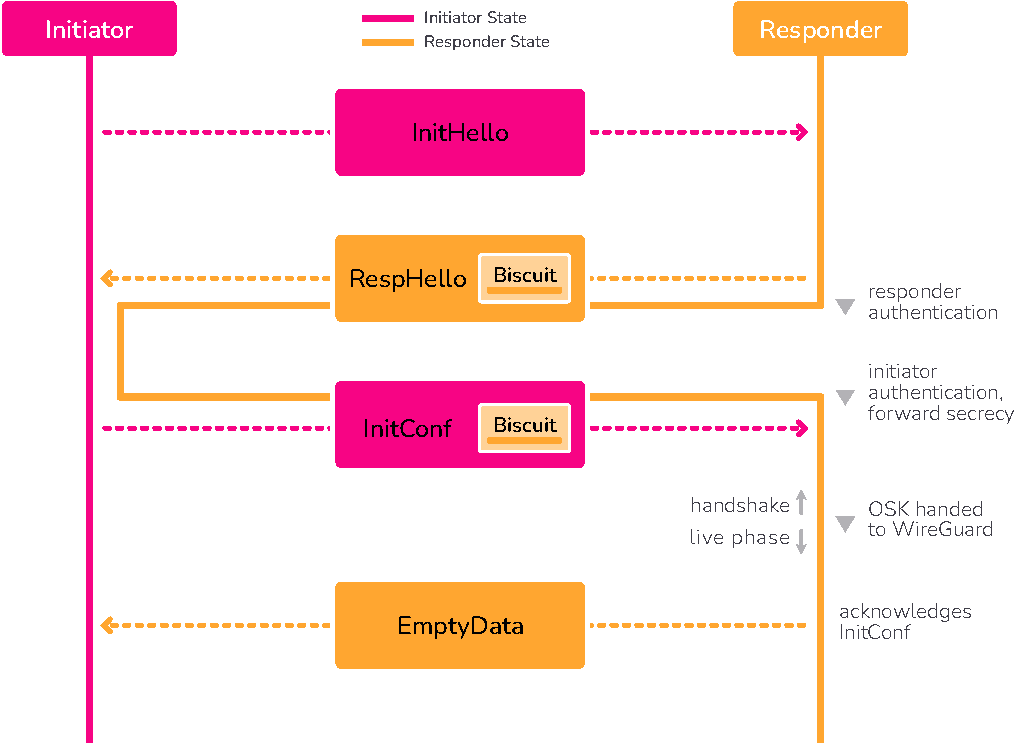
\includegraphics[width=\linewidth]{graphics/rosenpass-wp-key-exchange-protocol-rgb.pdf}
    \end{column}

    \begin{column}{.4\linewidth}
      \begin{itemize}
        \item Authenticated key exchange
        \item Three KEM operations interleaved to achieve mutual authentication and forward secrecy
        \item No use of signatures
        \item First package (InitHello) is unauthenticated
        \item Stateless responder to avoid disruption attacks
      \end{itemize}
    \end{column}
  \end{columns}
\end{frame}
